\documentclass{extbook}

% Paquetes
\usepackage[papersize={8.5in,11in},top=1in,bottom=1in]{geometry}
\usepackage[fontsize=11pt]{fontsize}
\RequirePackage{fix-cm}
\usepackage[T1]{fontenc}
\usepackage{lmodern}
\usepackage{fullpage}
\usepackage{titlesec}
\usepackage{parskip}
\usepackage{float}
\usepackage{array}
\usepackage{url}
\usepackage{hyperref}
\usepackage{graphicx}
\usepackage{tcolorbox}
\usepackage{tabularx}
\usepackage[dvipsnames]{xcolor}
\usepackage{titlesec}
\usepackage[utf8]{inputenc}
\usepackage{pifont} % \ding{51}, simbolo verificacion (flecha)

\DeclareUnicodeCharacter{2714}{\ding{51}} % ✔


\setcounter{tocdepth}{5}
\setcounter{secnumdepth}{5}

% Traducir palabras clave de inglés a español
\renewcommand{\contentsname}{Contenido}
\renewcommand{\figurename}{Figura}
\renewcommand{\listfigurename}{Lista de figuras}
\renewcommand{\bibname}{Bibliografía}
\renewcommand{\tablename}{Tabla}
\renewcommand{\listtablename}{Lista de tablas}


% Nuevos comandos
% Titulo del proyecto
\newcommand{\proyecto}{Desarrollo de Prototipo de Simulación Computacional de las Fases de la Luna: Una Herrameinta Interactiva para  la Educación y Divulgación Astronómica.}
\newcommand{\Proyecto}{\expandafter\MakeUppercase\expandafter{\proyecto}}

% Nombre de la universidad
\newcommand{\universidad}{Universidad Tecnológica de Panamá}
\newcommand{\Universidad}{\expandafter\MakeUppercase\expandafter{\universidad}}

% Nombre de la sede
\newcommand{\sede}{Veraguas}
\newcommand{\Sede}{\expandafter\MakeUppercase\expandafter{\sede}}

% Nombre de la facultad
\newcommand{\facultad}{Facultad de Ingeniería de Sistemas Computacionales}
\newcommand{\Facultad}{\expandafter\MakeUppercase\expandafter{\facultad}}

% Nombre de asesor
\newcommand{\asesor}{Edmanuel Cruz}
\newcommand{\Asesor}{\expandafter\MakeUppercase\expandafter{\asesor}}

% Datos estudiante
\newcommand{\elbin}{Elbin Puga}
\newcommand{\Elbin}{\expandafter\MakeUppercase\expandafter{\elbin}}
\newcommand{\cedulaep}{2-751-1082}

\newcommand{\arland}{Arland Barrera}
\newcommand{\Arland}{\expandafter\MakeUppercase\expandafter{\arland}}
\newcommand{\cedulaab}{9-763-400}

% Nombre del titulo
\newcommand{\titulo}{Licenciado en Ingeniería de Sistemas y Computación}
\newcommand{\Titulo}{\expandafter\MakeUppercase\expandafter{\titulo}}

% Nombre de la carrera
\newcommand{\carrera}{Licenciatura en Ingeniería de Sistemas y Computación}
\newcommand{\Carrera}{\expandafter\MakeUppercase\expandafter{\carrera}}


% Estilo de titulo de capitulo
% NOTE:
% Esto no se usa dado que se usa \section para evitar saltos de pagina
% salvo en la bibliografia, toc, tabla figuras y tablas
%
% NOTE:
% formato en la documentacion
% \titleformat{command}[shape]{format}{label}{sep}{before-code}[after-code]
%

\titleformat
  {\chapter} % Aplica a capitulos.
  [display] % Los mas parecido a un word?
  {\bfseries\huge\raggedright} % negrita, tamaño grande, alineación izquierda
  {} % Numero, subection, ... (no interesa)
  {0pt} % Espacio (vertical con display) entre etiqueta y título.
  {\vspace{-5cm}} % Espacio negativo hacia arriba (mas compacto).
  [\vspace{-1.5cm}] % Espacio entre titulo y texto del cuerpo (mas compacto).

  % Eliminar pagina doble extra al final de un capitulo
  \makeatletter
  \patchcmd{\chapter}
    {\if@openright\cleardoublepage\else\clearpage\fi}
    {\clearpage}
    {}{}
  \makeatother


% Inicio de documento
\begin{document}

% Registro oficial del tema de trabajo de graduación
\addcontentsline{toc}{section}{Registro oficial del tema de trabajo de graduación}
% Logo
\begin{minipage}{.1\textwidth} % ~10% ancho pagina
  \raggedright
  \center{
\includegraphics[scale=0.2]{Imagenes/fisc.png}}
\end{minipage}
\hfill
% Titulo
\begin{minipage}{.9\textwidth} % ~90% ancho pagina
  \raggedleft
  \centering
  {\bfseries
    \Universidad \\
    \Facultad \\
    REGISTRO OFICIAL DEL TEMA DE TRABAJO DE GRADUACIÓN
  }
\end{minipage}

\\
% Texto facultad
\begin{minipage}{.4\textwidth} % ~40% ancho pagina
  \raggedright
  \underline{Profesor(a)}\\
  VICEDECANO(A) ACADÉMICO(A)\\
  Facultad de Ingeniería de Sistemas\\
  Computacionales.
\end{minipage}
\hfill
% Tabla fecha, sede
\begin{minipage}{.6\textwidth} % ~60% ancho pagina
  \raggedleft
  \begin{tabular}{|c|c|c|c|c|c|c|}
    \hline
    \textbf{Fecha} & Día & \dd & Mes & \mm & Año & \aaaa \\
    \hline
    Sede & & \multicolumn{3}{c|}{Centro Regional} & \multicolumn{2}{c|}{\sede} \\
    \hline
  \end{tabular}
\end{minipage}

\\
\textbf{Estimado(a) Vicedecano(a):}

Por este medio le informamos que el Título del Trabajo de Graduación que he (hemos) escogido es:

\begin{tabularx}{\textwidth}{|X|}
  \hline
  \proyecto \\
  \hline
\end{tabularx}

EL mismo lleva como Objetivo General:

Desarrollar un prototipo de simulación computacional interactivo que represente de manera precisa las fases de la Luna, con el fin de mejorar la comprensión del fenómeno y promover la educación y divulgación astronómica.

El tema escogido tiene mayor relevancia en el área académica de: (ponderar en rangos de 5 a 1, donde 5 es para el departamento de mayor afinidad y 1 para el depatartamento de menor afinidad)

\begin{tabular}{|c|p{20em}|c|p{18em}|}
  \hline
  1 & Arquitectura y Redes de Computacionales & 5 & Computación y Simulación de Sistemas \\
  \hline
  5 & Ingeniería de Software & 4 & Programación de Computadoras \\
  \hline
  3 & \multicolumn{3}{l|}{\raggedright Sistemas de Información, Control y Evalación de Recursos Informáticos} \\
  \hline
\end{tabular}

Este trabajo de graduación lo consideramos de tipo:

% En esta tabla se emplea el simbolo unicode ✔ (verificado)
\begin{tabularx}{\textwidth}{|p{7em}|c|p{5em}|c|p{5em}|c|p{8.3em}|c|p{6em}|c|}
  \hline
  Teórico & & Teórico Práctico & ✔ & Práctica Profesional & & Certificación & & Otro & \\
  \hline
  \multicolumn{3}{|l|}{Si es Otro, especifique:} & \multicolumn{7}{c|}{} \\
  \hline
\end{tabularx}

Si es Práctica Profesional, Nombre de la Empresa:

\hspace*{2em} Para Optar por el Título de Licenciaura en: \small{\carrera}.\normalsize\\
\hspace*{2em} \underline{X}\\
Sugerimos como Asesor al Profesor(a): \asesor

El cual pertenece al Departamento Académico:\\
\underline{Departamento de Computación y Simulación de Sistemas}

\begin{tabularx}{\textwidth}{
  | p{7em}
  | p{5em}
  | p{7em}
  | p{11em}
  | >{\raggedright\arraybackslash}X |}
  \hline
  \textbf{NOMBRE} & \textbf{CÉDULA} & \textbf{TELÉFONOS} & \textbf{CORREO} & \textbf{FIRMA} \\
  \hline
  \estudianteuno & \cedulauno & \telefonouno & \correouno & \\
  \hline
  \estudiantedos & \cedulados & \telefonodos & \correodos & \\
  \hline
\end{tabularx}
\\
\itshape \small
Artículo 40 del Reglamento aprobado por el Consejo Académico: La Tesis será preferiblemente obra de un solo estudiante, pero por razones espaciales se permitirá más de un (1) estudiante es una misma Tesis.
\upshape \normalsize

% Columnas personalizadas b(big), s(small), t(tiny). Las 3 suman 100% ancho
\vfill
{
\renewcommand{\arraystretch}{1.5}
\newcolumntype{b}{>{\hsize=.45\hsize}X} % ~45% ancho pagina
\newcolumntype{s}{>{\hsize=.3\hsize}X} % ~30% ancho pagina
\newcolumntype{t}{>{\hsize=.25\hsize}X} % ~25% ancho pagina
\begin{tabularx}{\textwidth}{|s|b|t|}
  \hline
  Fecha: Nº\underline{X} & Fecha:\underline{X} & \\
  \hline
  \textbf{Vo. Bo. Prof. Asesor} & \textbf{Vo. Bo. Vicedecano(a) Académico} & \textbf{Vo. Bo. Decano} \\
  \hline
\end{tabularx}
}


% Formulario de verificación de entrega de documentos
\newpage
\addcontentsline{toc}{section}{Formulario de verificación de entrega de documentos}
% Titulo
{\bfseries \centering
\Universidad \\
\Facultad \\
VICEDECANATO ACADÉMICO \\
FORMULARIO DE VERIFICACIÓN DE ENTREGA DE DOCUMENTOS}

\vfill
{
\renewcommand{\arraystretch}{1.7}
% Tabla de formulario
\newcolumntype{b}{>{\hsize=.95\hsize}X} % ~95% ancho pagina
\newcolumntype{s}{>{\hsize=.05\hsize}X} % ~5% ancho pagina
\begin{tabularx}{\textwidth}{|s|b|}
  \hline
  ( ) & \begin{enumerate} \item[1.] Página de Presentación usando el formato respectivo. Nombre de la Universidad, Nombre de la Facultad, Título del Trabajo, Tipo de Trabajo, Nombre del Profesor Asesor, Integrante(s), Título a Optar, Año Elaboración. \end{enumerate} \\
  \hline
  ( ) & \begin{enumerate} \item[2.] Formulario de Registro Oficial del tema del trabajo de graduación firmado por el (los) estudiante(s) y el profesor Asesor propuesto. \end{enumerate} \\
  \hline
  ( ) & \begin{enumerate} \item[3.] Introducción. Incluye descripción de la situación actual, propuesto y las mejoras que el proyecto persigue. Debe incluir definición y alcance del tema, metodología y técnica de investigación a utilizar. \end{enumerate} \\
  \hline
  ( ) & \begin{enumerate} \item[4.] Índice del Anteproyecto \end{enumerate} \\
  \hline
  ( ) & \begin{enumerate} \item[5.] Objetivos (General y Específicos) \end{enumerate} \\
  \hline
  ( ) & \begin{enumerate} \item[6.] Plan de Contenido propuesto para el desarrollo del proyecto. \end{enumerate} \\
  \hline
  ( ) & \begin{enumerate} \item[7.] Bibliografía. Generalmente el mínimo son 10 referencias bibliográficas. Lo importante es que sea actualizado de acuerdo con el tema (por lo menos los últimos 5 años) \end{enumerate} \\
  \hline
  ( ) & \begin{enumerate} \item[8.] Cronograma de actividades. Presentado en diagrama de Gantt, preferiblemente en términos de meses o semanas. Los meses o semanas no deben ser etiquetados cronológicamente. \end{enumerate} \\
  \hline
  ( ) & \begin{enumerate} \item[9.] Herramientas de Software y Hardware que utilizar. \end{enumerate} \\
  \hline
  ( ) & \begin{enumerate} \item[10.] Créditos Académicos Oficiales y Formulario de Verificación de Requisitos para Trabajo de Graduación (Secretaría Académica) \end{enumerate} \\
  \hline
  ( ) & \begin{enumerate} \item[11.] Fotocopia de la constancia de matrícula del trabajo de graduación matriculado y el pago del seguro estudiantil por cada estudiante. La Matrícula debe cubrir el semestre o año académico en que se desarrolla el proyecto. \end{enumerate} \\
  \hline
  ( ) & \begin{enumerate} \item[12.] Información del Programa de Práctica Profesional (cuando sea el caso). \end{enumerate} \\
  \hline
\end{tabularx}
}

\vfill
REVISADO POR:\underline{\asesor} \hspace*{1em}FECHA:\underline{\dd/\mm/\aaaa}


% Portada
\newpage
{\bfseries \centering
\Universidad

\Facultad

\vspace{2em}

TÍTULO PROPUESTO DEL TRABAJO DE GRADUACIÓN

\Proyecto

\vspace{2em}

ANTEPROYECTO DE TRABAJO DE GRADUACIÓN

(TEÓRICO PRÁCTICO)

\vspace{3em}

ASESOR \\ \Asesor

\vspace{2em}

CO-ASESOR \\ JOSÉ CARLOS RANGEL

\vspace{2em}

ESTUDIANTES:

\Estudianteuno

\cedulauno

\Estudiantedos

\cedulados

\vspace{2em}

TRABAJO DE GRADUACIÓN PARA OPTAR AL TÍTULO DE \\ \Titulo

\vspace{4em}

AÑO \\ \aaaa

}


% Contenido preliminar
\tableofcontents
\listoffigures
\listoftables

\newpage
% Introduccion
\addcontentsline{toc}{section}{Introducción}
\section*{Introducción}
El campo de la astronomía es una ciencia que ha fascinado a la humanidad desde tiempos inmemoriales,
siendo la Luna uno de los objetos más estudiados y admirados. Las fases de la Luna, en particular,
no solo han sido motivo de observación y mitología, sino que también representan un fenómeno complejo
cuyo entendimiento resulta fundamental para diversas aplicaciones científicas y educativas.

A pesar de la relevancia de este fenómeno, la enseñanza tradicional de la astronomía en muchos contextos escolares
adolece de métodos interactivos y actualizados que faciliten la comprensión de conceptos tan abstractos como la mecánica celeste. 
Esta situación ha generado una brecha entre el conocimiento teórico y la práctica, afectando la calidad del aprendizaje en el área.

Ante esta problemática, la presente investigación propone el desarrollo de un prototipo de simulación computacional interactivo orientado 
a representar las fases de la Luna, con el fin de mejorar la comprensión del fenómeno y promover una educación más dinámica y participativa.


% Antecedentes
\addcontentsline{toc}{section}{Antecedentes}
\section*{Antecedentes}
\addcontentsline{toc}{subsection}{Compilación histórica del estudio astronómico}
\subsection*{Compilación histórica del estudio astronómico}
El estudio de los movimientos celestes ha sido una de las áreas fundamentales de la astronomía desde la antigüedad. 
Las civilizaciones mesopotámica, egipcia y maya registraron observaciones detalladas de la Luna y sus fases, utilizándolas para
la medición del tiempo y la elaboración de calendarios lunares \cite{antigua}.

La antigua civilización Maya, tenía conocimiento de la importancia y complejidad de la información
astronómica y calendárica. Esto indica que existía un contexto interpretativo especialmente prometedor que se 
fortaleció aun más tras la escritura jeroglífica proporcionando conocimiento clave del cielo y su aplicación social. Este conocimiento también
se reflejaba en un complejo sistema de contar meses lunares asociados a fechas escritas en la llamada cuenta larga que usaban para calcular y representar
el tiempo y pronto se dieron cuenta que podía servir para cálculos astronómicos \cite{maya}.


\begin{figure}[h]
    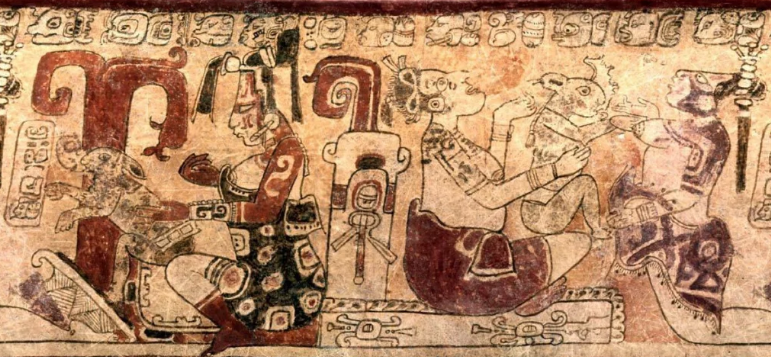
\includegraphics[scale = 0.7]{Imagenes/MayasMoon.png}
    \centering
    \caption{Puerta tallada de la diosa lunar Maya}{Fuente: Adaptado de \cite{ixchel}}
\end{figure}


Con el desarrollo del método científico, un gran exponente es Galileo Galilei quien es el precursor de la cosmología moderna ya que establecía
leyes sistemáticas capaces de ser observadas y expresadas en un lenguaje físico-matemático. Galileo mejoró el telescopio de la época y en sus observaciones
que son descritas en su libro "Sidereus Nuncius" \cite{sidereus} en 1610 establece que la Vía Láctea está compuesta por innumerables estrellas asociadas en complejos sistemas. En este texto se encuentran sus famosas observaciones telescópicas de la superficie lunar
y su anuncio del descubrimiento de cuatro satélites de Júpiter
(Ío, Europa, Ganímedes y Calixto), denominados por Galileo
“astros mediceos”


\begin{figure}[h]
    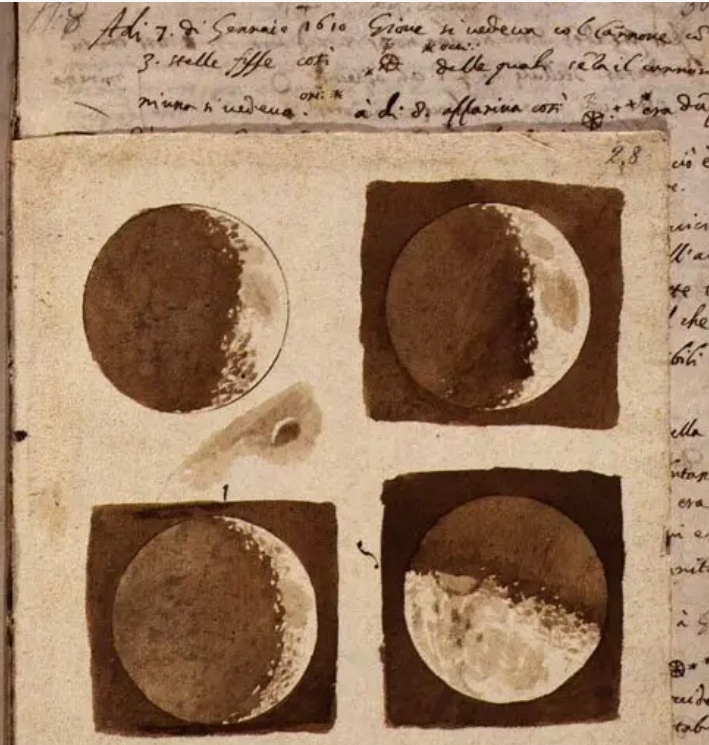
\includegraphics[scale = 0.5]{Imagenes/GalileoMoon.png}
    \centering
    \caption{Primeros dibujos de la Luna realizados por Galileo Galilei}{ Adaptado de: \cite{bbc}}

\end{figure}

\addcontentsline{toc}{subsection}{Historia de la simulación en la astronomía}
\subsection*{Historia de la simulación en la astronomía}

Los primeros modelos y representaciones que se tenían sobre la representación 
de fenomenos astronómicos se pueden encontrar en el papiro "Liber de coelo et mundo"
donde se aprecian diagramas geométricos relacionados con círculos y diámetros lo que da a entender
que el contenido estaba relacionado con astronomía y geometría esférica.

\begin{figure}[H]
    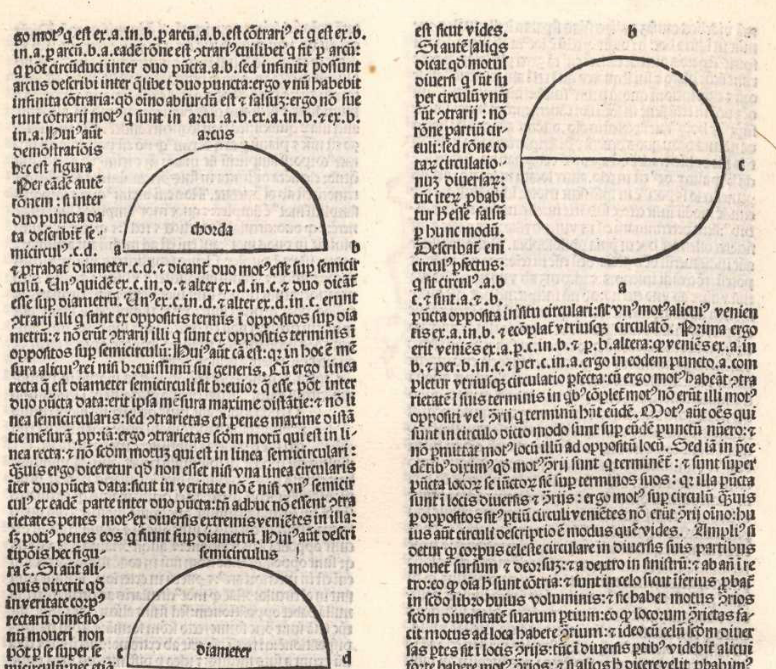
\includegraphics[scale = 0.55]{Imagenes/papiro.png}
    \centering
    \caption{Representación geométrica de cuerpos celestes}{ Adaptado de: \cite{decaelo}}
\end{figure}

También se destaca una curiosa representación de las fases de la luna en el año 1492 del capítulo `Liber de coelo et mundo' del libro `Introductiones in Aristotelis libros naturales' del teólogo francés y erudito griego Jacques Lefèvre d'Étaples.

\begin{figure}[H]
    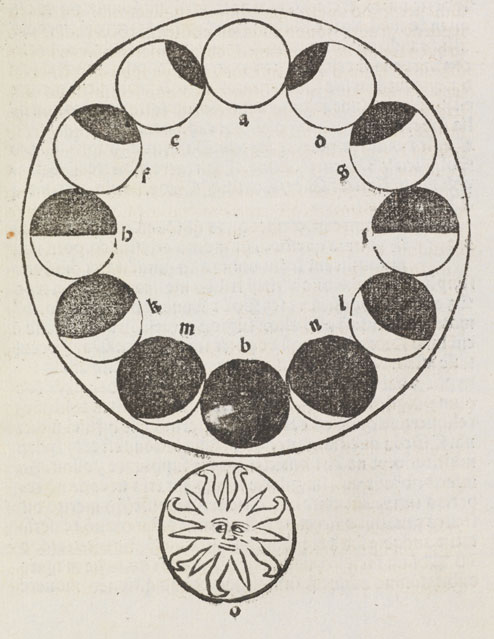
\includegraphics[width = 12cm, height=7.5cm]{Imagenes/fasesLunares1492.png}
    \centering
    \caption{Fases Lunares de Itroductiones in Aristotelis libros naturales}{ Adaptado de: \cite{lunarspine}}
\end{figure}

\addcontentsline{toc}{subsection}{Transición a la era digital}
\subsection*{Transición a la era digital}

Las simulaciones numéricas han permitido a los astrónomos estudiar procesos complejos que son inaccesibles mediante observación directa. 
Por ejemplo, con la llegada de telescopios de nueva generación como el Large Synoptic Survey Telescope (LSST) la astronomía ha entrado en la era del "Big Data". El LSST, por ejemplo, generará aproximadamente 15 terabytes de datos cada noche, lo que requiere el desarrollo de nuevas técnicas de análisis y almacenamiento de datos. Esto ha llevado al surgimiento de la astroinformática, una disciplina que combina la astronomía con la informática para manejar y analizar estos vastos conjuntos de datos\cite{huijse2014}.

También se puede encontrar que la visualización de datos astronómicos ha avanzado significativamente con el uso de tecnologías de realidad virtual (VR). Herramientas
como iDaVIE\cite{jarrett2021} permiten a los investigadores explorar datos astrofísicos en entornos inmersivos, facilitando una comprensión más intuitiva de estructuras complejas y relaciones espaciales en el cosmos. Esta metodología mejora la interpretación de datos y apoya el descubrimiento científico

Con estos antecedentes de la era digital con la integración de la computación en la astronomía ha permitido avances significativos en la simulación, análisis y visualización de fenómenos cósmicos, ampliando nuestra comprensión del universo y abriendo nuevas vías para la investigación científica.




Sin embargo, la mayoría de estas herramientas requieren hardware especializado o no permiten la consulta de datos astronómicos reales. 
Como respuesta a esta brecha, han surgido iniciativas basadas en software que utilizan cálculos precisos para predecir las fases de la Luna
en un intervalo de tiempo determinado, integrando modelos matemáticos y datos astronómicos provenientes de efemérides.

Estos avances han abierto nuevas posibilidades para la creación de recursos didácticos accesibles, que combinan precisión científica con representaciones visuales intuitivas.

% Estudios de investigación
\addcontentsline{toc}{section}{Estudios de investigación}
\section*{Estudios de investigación}
En esta sección, se aborda una revisión de literatura en aspectos de
nuestra área de investigación que comprende la astronomía y las fases de la luna
como objeto de estudio.
\addcontentsline{toc}{subsection}{La astronomía como ciencia}
\subsection*{La astronomía como ciencia}

En la revisión literaria podemos encontrar las siguientes definiciones de astronomía:

La astronomía es la ciencia natural del universo, en su
concepto más general. La astronomía
se dedica a estudiar las posiciones, distancias, movimientos, estructura y evolución de los astros y para ello se basa casi exclusivamente en la información
contenida en la radiación electromagnética o de partículas que alcanza al observador \cite{conceptos2009}


Es una disciplina que nos abre los ojos, da contexto a nuestro lugar en el universo y puede remodelar la idea de cómo vemos el mundo \cite{iau2025}.

En base a las definiciones presentadas, se puede afirmar que la astronomía se trata de una ciencia y disciplina fundamental
para comprender la estructura y evolución del universo, permitiendo grandes avances en conocimiento del universo.

La exploración de dicha ciencia, ha permitido comprender la formación y evolución de los cuerpos rocosos que están en nuestro sistema solar, así como el impacto de eventos astronómicos en la geología terrestre.

Dentro de ese campo, la luna es uno de los cuerpos más estudiados debido a su cercanía con la Tierra, además su influencia en nuestro planeta
como en aspectos físicos como formación de mareas hasta aspectos biológicos han sido tema de numerosos estudios.

\addcontentsline{toc}{subsection}{El fenómeno de las fases lunares}
\subsection*{El fenómeno de las fases lunares}


Estas fases están determinadas por las posiciones relativas cambiantes de la Luna, la Tierra y el Sol, que determinan qué parte de la superficie de la Luna está iluminada desde la perspectiva de la Tierra \cite{gullari2025}

En la tabla 4.1 se encuentran se aprecia detalladamente propiedades de este fenómeno astronómico:

\begin{table}[h]
    \centering
    \renewcommand{\arraystretch}{1.2} % Ajusta el espaciado entre filas
    \begin{tabular}{|l|c|p{7cm}|}
        \hline
        \textbf{Fase} & \textbf{\% Iluminación} & \textbf{Características Observables} \\
        \hline
        Luna Nueva & 0\% & Invisible desde la Tierra. \\
        \hline
        Luna Creciente & 1-49\% & Franja de luz en el lado derecho. \\
        \hline
        Cuarto Creciente & 50\% & La mitad derecha es visible. \\
        \hline
        Luna Gibosa Creciente & 51-99\% & Brillo creciente, casi llena. \\
        \hline
        Luna Llena & 100\% & Totalmente iluminada. \\
        \hline
        Luna Gibosa Menguante & 51-99\% & Brillo decreciente, luz en el lado izquierdo. \\
        \hline
        Cuarto Menguante & 50\% & La mitad izquierda es visible. \\
        \hline
        Luna Menguante & 1-49\% & Media luna antes de la luna nueva. \\
        \hline
    \end{tabular}
    \caption{Fases Lunares y Características Resumidas}
    \label{tabla:fases_lunares}
\end{table}

Para que se complete un ciclo completo de fases, la luna tarda aproximadamente 29,53 días. Esto ha sido fundamental en la creación de calendarios y ha influido en diversas culturas para determinar
festividades y actividades agrícolas.

\addcontentsline{toc}{subsection}{Evolución científica del estudio de la Luna}
\subsection*{Evolución científica del estudio de la Luna}

En el siglo XX, los estudios de la luna alcanzó su punto más exponencial con la misión de Apollo 11 en 1969, cuando
los astronautas Neil Armstrong y Buzz Aldrin se convirtieron en los primeros seres humanos en pisar la Luna.

Recientemente, misiones como  Lunar Reconnaissance Orbiter (LRO) y Chandrayaan-2 \cite{Singh2022} han proporcionado datos para
estudiar presencia de hielo en los polos lunares lo que permite explorar gracias a avances de la tecnología y simulaciones, las
características internas del satélite.

Se concluye en esta sección del área de investigación que la luna ha sido objeto de estudio y fascinación a lo largo de la historia. Sus fases han sido fundamentales para la creación de calendarios, mientras que su exploración ha impulsado el desarrollo tecnológico y científico. Comprender su fenómeno astronómico no solo amplía el conocimiento del sistema solar, sino que también sienta las bases para futuras misiones espaciales que podrían utilizar la Luna como punto de partida para la exploración interplanetaria.


\addcontentsline{toc}{subsection}{Importancia de la Simulación en el Estudio de Fenómenos Astronómicos}
\subsection*{Importancia de la Simulación en el Estudio de Fenómenos Astronómicos}

\addcontentsline{toc}{subsubsection}{Ámbito científico}
\subsubsection*{Ámbito científico}


En este ámbito, el grupo de investigación GPLA se desarrolló una serie de códigos escritos en
Python para la simulación de ondas electrostáticas uni- y bidimensionales \cite{ondas}. Esto se hizo para simular condiciones del plasma donde
no solo existan haces o haz y una especie de electrones en el universo.

Además, la importancia de la simulación proporciona la capacidad de modelary predecir el comportamiento de sistemas planetarios\cite{perryman}.

La idoneidad de Python como lenguaje de aplicaciones ha sido posible gracias a los grandes
progresos logrados en la última década en la mejora de las herramientas que permiten utilizarlo
de manera efectiva para manipular datos astronómicos \cite{green}.

En base a la literatura, se puede evidenciar que hay una gran importancia de realizar simulaciones en el estudio de fenómenos astronómicos
gracias a software vérsatil o incluso con la integración de lenguajes de programación como lo fue Python para la manipulación de grandes volumenes
de datos y su posterior simulación. La evolución de los lenguajes de programación ayudan a los científicos a analizar, estudiar, y representar datos astronómicos 
para modelar comportamientos astronómicos y obtener conclusiones que permitan desarrollar teorías científicas.



\addcontentsline{toc}{subsubsection}{Ámbito educativo}
\subsubsection*{Ámbito educativo}

El simulador Stellarium fue utilizado en cada sesión de 60 minutos por la educadora en la primera y tercera unidad. Se eligió esta herramienta ya que muestra el cielo nocturno y su evolución a lo largo del tiempo. En la primera unidad, esta herramienta permitió dar a conocer los niños y niñas las trayectorias que siguen los planetas en el cielo y los meses en los que pueden ser vistos. También señalar los movimientos de la luna y sus fases \cite{PerezLisboa2020}.

Los autores del trabajo previamente descrito, afirman que Las TIC, son un medio didáctico recreativo donde el profesor y el estudiante no solo interactúan con objetos inanimados, si no que se les puede generar movimiento, lo que es muy divertido para aprender y enseñar de una manera didáctica.

El uso de la Realidad Aumentada (RA) como una herramienta innovadora en la enseñanza de la astronomía. Desarrollado por el Instituto Nacional de Astrofísica de Italia (INAF), este proyecto implementa aplicaciones de RA para enriquecer la experiencia educativa, permitiendo a los estudiantes interactuar con modelos tridimensionales y obtener información adicional sobre diversos fenómenos astronómicos. Estas aplicaciones han sido distribuidas en escuelas y al público general a través de EduINAF, la revista en línea dedicada a la educación y divulgación científica \cite{nasa}. 
La integración de RA en el aprendizaje ha demostrado aumentar la motivación y comprensión de los estudiantes, ofreciendo oportunidades educativas únicas y fomentando una experiencia de aprendizaje más inmersiva y atractiva.

La revisión literaria nos indica que la integración de software de simulación en las escuelas, demuestra que se logra enseñar temas de astronomía de manera inmersa y a la vez fascinante lo cual hace
que el aprendizaje mediante simulación sea una opción recurrida a explicar fenómenos astronómicos con mayor claridad y didáctica.

En la revisión de literatura, podemos encontrar el simulador 
"Lunar Phase Simulator" de la Universidad de Nebraska-Lincoln’s. \cite{Ucar2014}

\begin{figure}[h]
    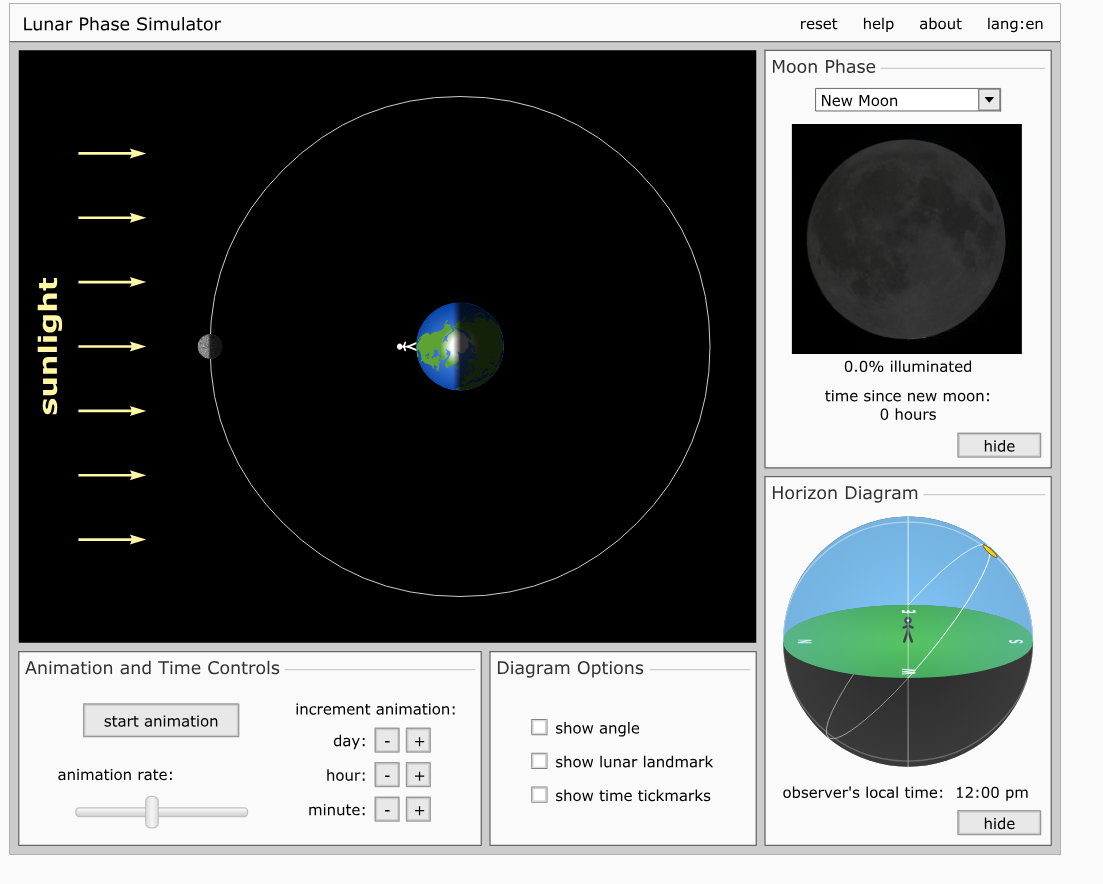
\includegraphics[scale = 0.5]{Imagenes/nebraska.png}
    \centering
    \caption{Simulador de fases de la luna}{Fuente: \cite{UNL2025}}
\end{figure}

\vspace{2em}
El simulador permite a los estudiantes comprender visualmente cómo la Luna cambia de fase al orbitar la Tierra, mostrando la relación entre la posición de la Luna, la Tierra y la luz solar. Para lograrlo, se emplea un frontend desarrollado con HTML, JavaScript y CSS, que incluye controles interactivamente ajustables para modificar el tiempo y observar en tiempo real el cambio de fases.

La representación visual abarca una simulación orbital en 2D, una vista desde el horizonte del observador y un indicador de fase lunar que muestra el porcentaje de iluminación. Como resultado, este recurso se presenta como una herramienta intuitiva y visualmente atractiva para la enseñanza en todos los niveles, no requiere conocimientos previos al basarse en la manipulación gráfica y resulta ideal para principiantes en astronomía.

\addcontentsline{toc}{subsection}{Análisis comparativo}
\subsection*{Análisis comparativo}

A continuación, se realiza una comparativa del simulador de la figura 5 con nuestra propuesta del prototipo:

\begin{table}[H]
    \centering
    \begin{tabular}{|p{4.5cm}|p{5.5cm}|p{5.5cm}|}
        \hline
        \textbf{Criterio} & \textbf{Lunar Phase Simulator (Nebraska)} & \textbf{Propuesta} \\
        \hline
        \textbf{Objetivo} & Visualizar fases lunares de forma interactiva. & Simulación científica con datos reales, material descargable y evaluación del aprendizaje. \\
        \hline
        \textbf{Interactividad} & El usuario ajusta la posición de la Luna manualmente. & El usuario ingresa fechas, obtiene gráficos y responde un \textbf{quiz interactivo} para reforzar el aprendizaje. \\
        \hline
        \textbf{Datos Adicionales} & No proporciona información numérica. & Muestra distancia Tierra-Luna, iluminación y visibilidad, además de permitir la autoevaluación. \\
        \hline
        \textbf{Exportación de Datos} & No permite guardar información. & Genera reportes en PDF para estudiantes con sus resultados del quiz y gráficos de fases lunares. \\
        \hline
        \textbf{Aplicabilidad Educativa} & Bueno para principiantes en astronomía. & Útil tanto para estudiantes como para investigadores, incorporando \textbf{evaluación y retroalimentación} del aprendizaje. \\
        \hline
    \end{tabular}
    \caption{Comparación entre el Lunar Phase Simulator (Nebraska) y la propuesta del prototipo, incluyendo evaluación interactiva.}
    \label{tab:comparacion}
\end{table}


% Propuesta
\addcontentsline{toc}{section}{Propuesta}
\section*{Propuesta}
El impacto en la educación científica afecta la comprensión general de la astronomía.

Basándonos en el trabajo de Jordi Solbes y Rafael Palomar \cite{aprendizajeEscuelas}, concluyen que la mayoría de estudiantes en un colegio de España,
no comprenden y/o desconocen aspectos básicos de la astronomía pese a una reiterada enseñanza de la misma.

Además, confirman que un 6.2\% del alumnado sería capaz orientarse de día y noche y la sorpresa es que ningún estudiante es capaz de explicar las 
fases de la luna.

\begin{table}[H]
  \centering
  \begin{tabular}{p{25em}c}
    \hline
    Categoría & Porcentaje \\
    \hline
    NS/NC & 23.9\% \\
    Respuestas incorrectas & 76.1\% \\
    Explica las fases de la Luna correctamente & 0\% \\
    \hline
  \end{tabular}
  \caption{Porcentajes según puntuacion cuestionario alumnos}{Adaptado de: \cite{aprendizajeEscuelas}}
  \label{tab:cuestionario}
\end{table}

Si nos basamos en el trabajo de Loyola y Ortega \cite{rabanales2021}, podemos extraer una tabla sobre una prueba realizada a alumnos en Chile sobre las fases de la luna

\begin{table}[H]
  \centering
  \begin{tabular}{|c|c|c|c|c|}
    \hline
    \multirow{2}{10em}{\centering Dimensión \\ (Nº pregunta del test)} & \multicolumn{2}{c|}{Octavo básico} & \multicolumn{2}{c|}{Cuarto medio} \\
    \cline{2-5}
    & Incorrectas & Correctas & Incorrectas & Correctas \\
    \hline
    Fases de la Luna (8-10) & 79.2\% & 20.8\% & 63.3\% & 36.7\% \\
    \hline
  \end{tabular}
  \caption{Porcentaje de respuestas correctas e incorrectas en el test, sobre Fases de la Luna}{Adaptado de: \cite{rabanales2021}}
  \label{tab:test}
\end{table}

Aunque no encontramos literatura que muestre datos acerca del nivel de conocimientos
en escuelas ya sea premedia y media en Panamá, sería una buena idea realizar ese estudio para tener un registro
de las nociones tendrían los estudiantes en el área de astronomía. 

Tomando en cuenta los trabajos anteriormente mencionados, podemos identifica que la forma en que se enseña la astronomía y un tema básico como el fenómeno de las fases de la luna, continúa presentándose de manera abstracta y poco
interactiva en muchos entornos educativos. Los métodos tradicionales, basados en explicaciones teóricas y representaciones estáticas, no permiten al estudiante visualizar
ni experimentar de manera dinámica la interacción entre la Tierra, la Luna y el Sol. Esta carencia de herramientas interactivas genera dificultades para comprender la esencia 
del fenómeno, reduciendo el interés y la motivación tanto de estudiantes como de docentes. 

En consecuencia, se identifica el problema principal: \textbf{la ausencia de un recurso didáctico 
basado en tecnología interactiva que facilite el aprendizaje y la divulgación de los procesos astronómicos relacionados con las fases lunares.}


% Objetivo general
\addcontentsline{toc}{section}{Objetivo General}
\section*{Objetivo General}
Desarrollar un prototipo de simulación computacional interactivo que represente de manera precisa las fases de la Luna, con el fin de mejorar la comprensión del fenómeno y promover la educación y divulgación astronómica.

% Objetivos especificos
\addcontentsline{toc}{section}{Objetivos Específicos}
\section*{Objetivos Específicos}
\begin{itemize}
    \item Investigar y recopilar los factores que afectan negativamente el aprendizaje de la astronomía en el entorno escolar, analizando tanto aspectos metodológicos como la disponibilidad de recursos y herramientas didácticas.
    \item Diseñar y desarrollar un prototipo de software utilizando herramientas de código abierto (por ejemplo, Python y sus librerías asociadas) que permita simular de forma interactiva las fases lunares.
    \item Implementar una interfaz gráfica amigable e intuitiva que facilite la interacción del usuario, permitiendo la modificación de parámetros y la visualización en tiempo real de los cambios en las fases de la Luna.
\end{itemize}



% Metodologia
\addcontentsline{toc}{section}{Metodología}
\section*{Metodología}
Se plantea una metodología investigación-acción para el desarrollo del prototipo, que combina la acción y la reflexión en un proceso cíclico e iterativo. En la fase inicial se realizará una exhaustiva investigación y análisis de los fundamentos astronómicos relacionados con las fases de la Luna, consultando fuentes académicas, libros especializados y bases de datos científicas. Durante esta etapa se identificarán las variables clave y se definirán los parámetros que deben ser simulados, permitiendo comprender a fondo tanto el fenómeno como las necesidades educativas asociadas.

Con la información recopilada, se procederá a la planificación y diseño del prototipo. Aquí se definirá la arquitectura del software y la interfaz de usuario, apoyándose en diagramas y herramientas como UML para plasmar la estructura del sistema. Se seleccionarán tecnologías y lenguajes de programación adecuados—por ejemplo, Python y JavaScript—que permitan integrar gráficos interactivos y simulaciones en tiempo real, facilitando la interacción del usuario mediante el ajuste de parámetros como el ángulo de visión o la posición relativa de la Tierra y la Luna.

La fase de acción consistirá en la implementación del prototipo, donde se integrarán algoritmos matemáticos con elementos gráficos mediante un proceso de codificación modular. Se aplicarán pruebas unitarias e integradas para garantizar la precisión y estabilidad del sistema, y se documentará de forma continua el desarrollo, estableciendo mecanismos de control de versiones que permitan incorporar mejoras de manera iterativa.

Finalmente, se llevará a cabo una fase de evaluación y retroalimentación, característica de la investigación - acción. En esta etapa, el prototipo se pondrá a disposición de expertos en astronomía y educación, tanto a nivel nacional como internacional, para recibir observaciones críticas y sugerencias. Los resultados obtenidos serán objeto de reflexión y análisis, lo que posibilitará ajustar y refinar el prototipo en nuevos ciclos de acción. Este enfoque cíclico no solo asegura la solución de los problemas identificados, sino que también fomenta la generación de nuevo conocimiento y la continua optimización del recurso didáctico.


% Delimitacion
\addcontentsline{toc}{section}{Delimitación}
\section*{Delimitación}
Esta investigación se centra en el desarrollo de un prototipo de simulación computacional interactivo para representar las fases de la luna. Se delimita exclusivamente a este fenómeno dentro del área de astronomía, sin abordar otros aspectos o fenómenos astronómicos. Además, se orienta a entornos educativos donde la comprensión de las fases lunares presenta desafíos, limitando el estudio al análisis y propuesta de soluciones para mejorar la enseñanza y divulgación de este tema en particular.

% Justificacion
\addcontentsline{toc}{section}{Justificación}
\section*{Justificación}
La propuesta se fundamenta en la necesidad de innovar los métodos de enseñanza de la astronomía, abordando esa existente brecha entre la teoría y la práctica. El uso de simulaciones interactivas permite a los usuarios experimentar de manera directa con los conceptos astronómicos, facilitando el aprendizaje mediante la visualización y manipulación de variables en tiempo real. Esto no solo mejora la comprensión del fenómeno de las fases de la Luna, sino que también fomenta un aprendizaje activo y participativo.

Además, el desarrollo de un prototipo basado en software de código abierto garantiza una solución de bajo costo y alta accesibilidad, lo cual es especialmente relevante para instituciones educativas con recursos limitados. 


% Estrucutra de la memoria
\addcontentsline{toc}{section}{Estructura de la memoria}
\section*{Estructura de la memoria}
La estructura de la memoria se plantea de la siguiente manera:

El \textbf{Capítulo I} consiste en las generalidades del proyecto, objetivos e importancia del desarrollo de este. En el \textbf{Capítulo II} se describirán las técnicas que se utilizaran en el proyecto, de igual forma se presentan la actualidad de los sistemas de simulación de las Fases de la Luna. El \textbf{Capítulo III} presenta las tecnologías con las que se realizará el proyecto. En el \textbf{Capítulo IV} se describirá el desarrollo del sistema propuesto.

En el \textbf{Capítulo V} se expondrán las configuraciones de los experimentos y sus resultados obtenidos del proyecto. Finalmente, las conclusiones serán presentadas en el \textbf{Capítulo VI}. Al final del documento se mostrarán las referencias bibliográficas utilizadas para el desarrollo del proyecto y los anexos.


% Plan de contenido
\addcontentsline{toc}{section}{Plan de contenido}
\section*{Plan de contenido}
\begin{enumerate}
  \item[I.] Dedicatoria
  \item[II.] Agradecimiento
  \item[III.] Índice General
  \item[IV.] Índice de tablas y figuras
\end{enumerate}

\vspace{1em}
CAPÍTULO 1. Generalidades del proyecto
\begin{enumerate}
  \item[1.1 -] Antecedentes
  \begin{enumerate}
    \item[1.1.1 -] Compilación histórica del estudio astronómico
    \item[1.1.2 -] Historia de la simulación en la astronomía
    \item[1.1.3 -] Transición a la era digital
  \end{enumerate}
  \item[1.2 -] Identificación del problema
  \item[1.3 -] Objetivo General
  \item[1.4 -] Objetivos Específicos
  \item[1.5 -] Justificación
  \item[1.6 -] Delimitación
\end{enumerate}

\vspace{1em}
CAPÍTULO 2. Marco Teórico
\begin{enumerate}
  \item[2.1 -] Área de investigación
  \begin{enumerate}
    \item[2.1.1 -] La astronomía como ciencia
    \item[2.1.2 -] El fenómeno de las fases lunares
    \item[2.1.3 -] Evolución científica del estudio de la Luna
    \item[2.1.4 -] Importancia de la Simulación en el Estudio de Fenómenos Astronómicos
    \begin{enumerate}
      \item[2.1.4.1 -] Ámbito científico
      \item[2.1.4.2 -] Ámbito educativo
    \end{enumerate}
  \end{enumerate}
  \item[2.2 -] Proyectos Similares
  \begin{enumerate}
    \item[2.2.1 -] Análisis comparativo
  \end{enumerate}
  \item[2.3 -] Tecnologías de desarollo
  \begin{enumerate}
    \item[2.3.1 -] Lenguaje de programación
    \item[2.3.2 -] Librerías y Frameworks
    \item[2.3.3 -] Cálculo y Simulación Astronómica
    \item[2.3.4 -] Visualización de Datos
    \item[2.3.5 -] Desarrollo Web e Interfaz Gráfica
    \item[2.3.6 -] Generación de Reportes
    \item[2.3.7 -] Justificación del Uso de Estas Herramientas
    \item[2.3.8 -] Plataformas y Entornos de Desarrollo
    \item[2.3.9 -] Beneficios del Uso de Software de Código Abierto   
  \end{enumerate}
\end{enumerate}

\vspace{1em}
CAPÍTULO 3. Propuesta del Proyecto
\begin{enumerate}
  \item[3.1 -] Metodología del trabajo
  \item[3.2 -] Escenario de aplicación
  \item[3.3 -] Cronograma de actividades
  \item[3.4 -] Presupuesto Real
  \item[3.5 -] Diseño Conceptual
\end{enumerate}

\vspace{1em}
CAPÍTULO 4. Prototipo del Proyecto
\begin{enumerate}
  \item[4.1 -] Interfaces del sistema
  \item[4.2 -] Módulos Desarrollados
  \item[4.3 -] Construcción del prototipo
\end{enumerate}

\vspace{1em}
CAPÍTULO 5. Resultados
\begin{enumerate}
  \item[5.1 -] Resultados
\end{enumerate}

\vspace{1em}
CAPÍTULO 6. Conclusiones
\begin{enumerate}
  \item[6.1 -] Conclusiones
\end{enumerate}

\vspace{1em}
BIBLIOGRAFÍA


% Herramientas de hardware y software a utilizar
\addcontentsline{toc}{section}{Herramientas de hardware y software a utilizar}
\section*{Herramientas de hardware y software a utilizar}
\addcontentsline{toc}{subsection}{Lenguaje de programación}
\subsection*{Lenguaje de programación}
Para el desarrollo de la propuesta del prototipo, se implemetará el lenguaje de programación Python debido 
a su ámbito en área científica y su integración en la Web.

\begin{figure}[H]
    
\includegraphics[scale = 0.80]{Imagenes/python-logo.png}
    \centering
    \caption{Logo de Python}{Fuente: Adaptado de Internet}
\end{figure}

\begin{itemize}
    \item \textbf{Facilidad de uso:} Python es un lenguaje de alto nivel con una sintaxis clara y legible, lo que facilita el desarrollo y mantenimiento del código.
    \item \textbf{Disponibilidad de librerías:} Posee una amplia gama de librerías especializadas en cálculo astronómico, visualización y desarrollo web.
    \item \textbf{Comunidad de soporte:} Python cuenta con una de las comunidades de desarrolladores más grandes, lo que garantiza una amplia documentación y soporte técnico.
\end{itemize}

\addcontentsline{toc}{subsection}{Librerías y Frameworks}
\subsection*{Librerías y Frameworks}

El desarrollo del prototipo utilizará diversas \textbf{librerías y frameworks} que contribuyen a la precisión y eficacia de la simulación:

\addcontentsline{toc}{subsection}{Cálculo y Simulación Astronómica}
\subsection*{Cálculo y Simulación Astronómica}
\begin{itemize}
    \item \textbf{Skyfield:} Permite calcular posiciones astronómicas con alta precisión, incluyendo las fases de la Luna basadas en efemérides oficiales de la NASA.
    \item \textbf{NumPy:} Facilita operaciones numéricas eficientes para manejar datos astronómicos.
\end{itemize}

\addcontentsline{toc}{subsection}{Visualización de Datos}
\subsection*{Visualización de Datos}
\begin{itemize}
    \item \textbf{Matplotlib:} Utilizado para generar gráficos que representen la evolución de las fases de la Luna de manera precisa y clara.
    \item \textbf{Plotly:} Posible alternativa para gráficos interactivos en la interfaz web.
\end{itemize}

\addcontentsline{toc}{subsection}{Desarrollo Web e Interfaz Gráfica}
\subsection*{Desarrollo Web e Interfaz Gráfica}
\begin{itemize}
    \item \textbf{Flask:} Framework ligero en Python para manejar la lógica del servidor y comunicación con la interfaz de usuario.
    \item \textbf{HTML, CSS y JavaScript:} Tecnologías fundamentales para la creación de la interfaz web interactiva.
\end{itemize}

\addcontentsline{toc}{subsection}{Generación de Reportes}
\subsection*{Generación de Reportes}
\begin{itemize}
    \item \textbf{ReportLab:} Permite la generación de archivos PDF para que los usuarios descarguen información detallada sobre las fases de la Luna.
\end{itemize}

\addcontentsline{toc}{subsection}{Justificación del Uso de Estas Herramientas}
\subsection*{Justificación del Uso de Estas Herramientas}
\begin{itemize}
    \item \textbf{Skyfield} asegura precisión astronómica al basarse en datos de efemérides.
    \item \textbf{Matplotlib y Plotly} permiten representar gráficamente los cambios en las fases lunares de manera comprensible.
    \item \textbf{Flask + HTML/CSS/JavaScript} garantizan una interfaz intuitiva y accesible desde cualquier navegador.
    \item \textbf{por definir***} proporciona material educativo en PDF, facilitando la revisión posterior por parte de los estudiantes.
\end{itemize}

\addcontentsline{toc}{subsection}{Plataformas y Entornos de Desarrollo}
\subsection*{Plataformas y Entornos de Desarrollo}

Para el desarrollo del prototipo, se utilizarán las siguientes herramientas:

\begin{itemize}
    \item \textbf{Entorno de Desarrollo Integrado (IDE):} Se usa \textbf{VS Code} o \textbf{PyCharm}, ambos con soporte para Python y depuración eficiente.
    \item \textbf{Control de Versiones:} Git y GitHub serán empleados para gestionar cambios en el código y colaboración entre desarrolladores.
    \item \textbf{Entorno Virtual:} Se utilizará \texttt{venv} o \texttt{conda} para administrar dependencias y evitar conflictos entre librerías.
\end{itemize}

\addcontentsline{toc}{subsection}{Beneficios del Uso de Software de Código Abierto}
\subsection*{Beneficios del Uso de Software de Código Abierto}
\begin{itemize}
    \item Facilita la replicación y ampliación del proyecto por otros investigadores o educadores.
    \item Reduce costos al evitar el uso de licencias propietarias.
    \item Permite contribuciones de la comunidad para mejorar la simulación.
\end{itemize}



% Bibliografia
\addcontentsline{toc}{section}{Bibliografía}
\begin{thebibliography}{99}

\bibitem{antigua}
\textit{C. Ruggles and G. Urton, *Skywatching in the Ancient World: New Perspectives in Cultural Astronomy*. Boulder, CO: University Press of Colorado, 2007.}

\bibitem{maya} \textit{Stanislaw Iwaniszewski, Arqueología Mexicana, "Los ciclos lunares y el calendario maya".}  [Online]. Disponible: \url{https://arqueologiamexicana.mx/mexico-antiguo/los-ciclos-lunares-y-el-calendario-maya}

\bibitem{ixchel} \textit{C. Carcavilla, "Trabajo de Fin de Grado Arqueología UCM: La diosa Ix Chel en los mayas prehispánicos", 2022} Disponible: \url{https://www.researchgate.net/publication/363582211_Trabajo_de_Fin_de_Grado_Arqueologia_UCM_La_diosa_Ix_Chel_en_los_mayas_prehispanicos}.

\bibitem{sidereus} \textit{G. Galilei, *Sidereus Nuncius*. Venice, Italy: Thomas Baglioni, 1610. [Online]. Available}: \url{https://archive.org/details/sidereus_nuncius_202004/page/n9/mode/2up}. [Accessed: Feb. 9, 2025].

\bibitem{bbc} \textit{BBC Mundo, "La sorprendente revelación sobre la Luna y su evolución", Dec. 2, 2017. [Online]. Available:} \url{https://www.bbc.com/mundo/noticias-42202220}. [Accessed: Feb. 9, 2025].

\bibitem{decaelo} \textit{A. Magno and H. Mitanuni, *De caelo et mundo*. Venice, Italy: Impressum Uenetijs per Joannem de Forliuio, et Gregorium fratres, Nov. 1490. [Online]. Available:} \url{http://hdl.handle.net/10481/16176}. [Accessed: Feb. 9, 2025].

\bibitem{lunarspine} ResearchGate, 
``The influence of lunar phases and zodiac sign ‘Leo’ on perioperative complications and outcome in elective spine surgery,'' 
Scientific Figure, 2025. Disponible en: \href{https://www.researchgate.net/figure/Woodcut-from-1492-illustrating-the-lunar-phases-from-the-chapter-Liber-de-coelo-et_fig1_301581818}{ResearchGate}. [Accedido: 10 Feb. 2025].


\bibitem{huijse2014} P. Huijse, P. A. Estevez, P. Protopapas, J. C. Principe, y P. Zegers, 
``Computational Intelligence Challenges and Applications on Large-Scale Astronomical Time Series Databases,'' 
\textit{IEEE Computational Intelligence Magazine}, vol. 9, no. 3, pp. 27–39, 2014. \url{https://arxiv.org/pdf/1509.07823}

\bibitem{jarrett2021} T. H. Jarrett, A. Comrie, L. Marchetti, A. Sivitilli, S. Macfarlane, F. Vitello, U. Becciani, A. R. Taylor, J. M. van der Hulst, P. Serra, N. Katz y M. E. Cluver, 
``Exploring and interrogating astrophysical data in virtual reality,'' 
\textit{Astronomy and Computing}, vol. 37, p. 100502, 2021. 
DOI: \url{https://doi.org/10.1016/j.ascom.2021.100502}.

\bibitem{aprendizajeEscuelas} \textit{Solbes and R. Palomar, “Dificultades en el aprendizaje de la astronomía en secundaria”, Rev. Bras. Ensino Fís., vol. 35, no. 1, pp. 01–12, Jan. 2013, doi: 10.1590/S1806-11172013000100016.}

\bibitem{rabanales2021} F. Rabanales Loyola y C. Vanegas Ortega, 
``Concepciones alternativas sobre astronomía en estudiantes de educación básica y media de la Región Metropolitana de Chile,'' 
\textit{Estudios Pedagógicos (Valdivia)}, vol. 47, no. 2, pp. 247–268, 2021.

\bibitem{conceptos2009} J. Alfonso Garzón, D. Galadí Enríquez, y C. Morales Durán, Eds., \textit{100 Conceptos Básicos de Astronomía. Madrid, España: Instituto Nacional de Técnica Aeroespacial (INTA), 2009}

\bibitem{iau2025} Marissa Rosenberg, Pedro Russo, Unión Astronómica Internacional, 
\textit{Astronomía en la vida cotidiana}. [En línea]. Disponible en: \href{https://www.iau.org/public/themes/astronomy_in_everyday_life/spanish/}{https://www.iau.org/public/themes/astronomy\_in\_everyday\_life/spanish/}.

\bibitem{gullari2025} J. K. Gullari, 
\textit{The Impact of Moon Phases on Earth, Plants, and Humans: A Comprehensive Study from Project Alpha}, 
Jan. 9, 2025.

\bibitem{Singh2022}
A.~Singh, A.~Sharma, S.~Kumar, L.~Chang, A.~Vashishtha, R.~Raj, S.~Agrawal, and P.~Chauhan, ``\textit{Dielectric characterization and polarimetric analysis of lunar north polar crater Hermite-A using Chandrayaan-1 Mini-SAR, Lunar Reconnaissance Orbiter (LRO) Mini-RF, and Chandrayaan-2 DFSAR data},'' \textit{Advances in Space Research}, vol.~70, no.~12, pp.~4030--4055, 2022. doi: 10.1016/j.asr.2022.04.059.


\bibitem{ondas} \textit{L. D. Herrera and C. R. Arias Simulación de ondas generadas en la inestabilidad two-stream para
plasmas electrostáticos usando particle-in-cell simulación de ondas generadas en la inestabilidad
two-stream para plasmas electrostáticos usando particle-in-cell, 2019.}

\bibitem{perryman}\textit{M. Perryman, The Exoplanet Handbook. 2011. [Online]. Available: } \url{https://assets.cambridge.org/97805217/65596/frontmatter/9780521765596_frontmatter.pdf}


\bibitem{green} \textit{Greenfield, P., “What Python Can Do for Astronomy”, in <i>Astronomical Data Analysis Software and Systems XX</i>, 2011, vol. 442, p. 425.}

\bibitem{PerezLisboa2020}
S.~Pérez-Lisboa, C.~G. Ríos-Binimelis, and J.~Castillo Allaria, ``\textit{Realidad Aumentada y simuladores: astronomía para niños y niñas de cinco años},'' \textit{ALTERIDAD. Revista de Educación}, vol.~15, no.~1, pp.~25--35, 2020. doi: 10.17163/alt.v15n1.2020.02.


\bibitem{nasa} \textit{Leonardi, L., Daricello, L., and Giacomini, L., “Learning astronomy through Augmented Reality: EduINAF resources to enhance students' motivation and understanding”}  Art. no. EPSC2021-530, 2021. doi:10.5194/epsc2021-530.

\bibitem{Ucar2014}
S.~Uçar, ``\textit{The effects of simulation-based and model-based education on the transfer of teaching with regard to Moon phases},'' \textit{Journal of Baltic Science Education}, vol.~13, no.~3, pp.~327--338, 2014.

\bibitem{UNL2025} 
University of Nebraska-Lincoln, 
``\textit{Lunar Phases Simulator},'' 
[Online]. Available: \href{https://astro.unl.edu/naap/lps/animations/lps.html}{https://astro.unl.edu/naap/lps/animations/lps.html}. 
[Accessed: 11-Feb-2025].


\end{thebibliography}


% Cronograma de actividades
% NOTE: Usar otro programa para crear el cronograma, complicado en LaTeX
%
\addcontentsline{toc}{section}{Cronograma de actividades}
\section*{Cronograma de actividades}
\begin{figure}[H]
  \centering
  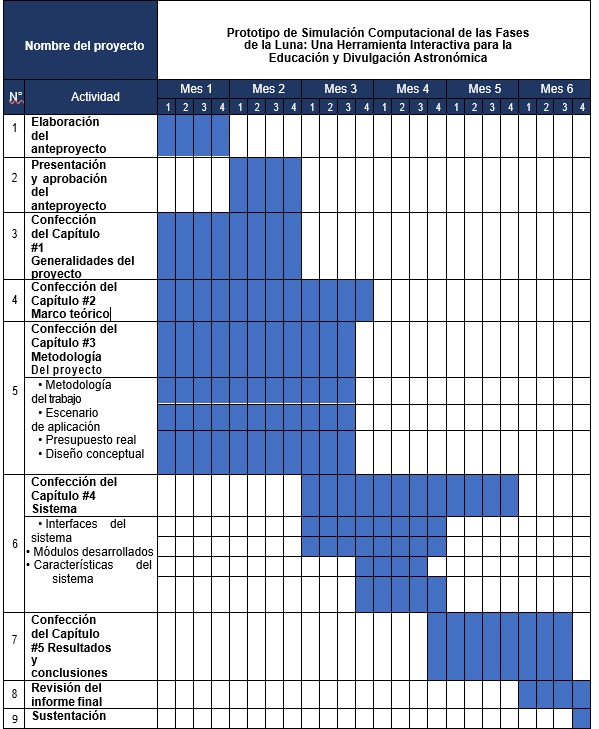
\includegraphics[scale=0.9]{Imagenes/cronograma.png}
  \caption{Cronograma de actividades}{Fuente: Propia}
\end{figure}


\end{document}
